%************************************************
\chapter{Quantum computing e machine learning}\label{ch:teoria}
%************************************************

% \emph{
%     Si noti che tutti i concetti introdotti nelle sezioni 2.1 e 2.2 possono essere trovati in 
%     qualunque libro di testo di base sull'informazione quantistica e quindi non ci saranno 
%     riferimenti individuali ad essi. Entrambe queste sezioni sono principalmente basate sul libro 
%     di testo di Noson e Mannucci\cite{noson}.
% }

Nella sezione \ref{sec:quantum_computing} si discuteranno i concetti fondamentali su 
cui si base il funzionamento di un quantum computer. 
L'unità di base di un computer classico è il bit e l'unità di base di 
un computer quantistico è una generalizzazione del concetto di bit, 
chiamato qubit, che sarà discussa in sezione \ref{sec:qubit}. 
Nella sezione \ref{sec:porte_quantistiche} si presentano le porte 
logiche quantistiche, che permettono di manipolare i qubit. 
Infine, in sezione \ref{sec:decoerenza} si discuterà di uno dei nuovi problemi con 
cui si deve avere a che fare quando si lavora con oggetti quantomeccanici, ovvero 
la decoerenza. 

Successivamente, in sezione \ref{sec:machine_learning}, verrà introdotta brevemente 
la branca del machine learning, spiegando il funzionamento dell'algoritmo k-nearest neighbours, 
per poi discuterne la versione quantistica in sezione \ref{sec:qml}. 

\section{Quantum computing} \label{sec:quantum_computing}

\subsection{Bit e qubit} \label{sec:qubit}

\begin{definition}
    Un bit è un'unità di informazione che descrive un sistema classico 
    bidimensionale. 
\end{definition}
I due possibili stati di un bit sono generalmente scritti come 
0 e 1, o meglio, nel nostro caso $\ket{0}$ e $\ket{1}$. 
Usando una notazione matriciale, possiamo rappresentare questi due 
stati come 
\begin{equation}
    \ket{0} = \begin{matrix}
        0 \\ 1
    \end{matrix}
    \begin{pmatrix}
        1 \\ 0
    \end{pmatrix}, \quad
    \ket{1} = \begin{matrix}
        0 \\ 1
    \end{matrix}
    \begin{pmatrix}
        0 \\ 1
    \end{pmatrix},
\end{equation}
dove i numeri a margine delle matrici indicano a quale stato si 
riferisce un determinato elemento di base. Poiché queste due 
rappresentazioni sono ortogonali, abbiamo che il bit che 
può trovarsi in uno stato tra $\ket{0}$ e $\ket{1}$. 

\begin{definition}
    Un bit quantistico o qubit è un'unità di informazione che descrive 
    un sistema quantistico bidimensionale. 
\end{definition}
Si rappresenterà il qubit come una matrice $2\times1$ a valori complessi 
\begin{equation}
    \begin{matrix}
        0 \\ 1
    \end{matrix}
    \begin{pmatrix}
        c_0 \\ c_1
    \end{pmatrix},
\end{equation}
dove $|c_0|^2 + |c_1|^2 = 1$. Si noti che un bit classico è un caso particolare 
di qubit. $|c_0|^2$ va interpretata come la probabilità che dopo una misura del 
qubit, questo sarà trovato nello stato $\ket{0}$. $|c_1|^2$ va interpretata come 
la probabilità che dopo una misura del qubit, questo sarà trovato nello stato 
$\ket{1}$. Allorquando si misura lo stato di un qubit, questo diventa automaticamente 
un bit. Quindi non "vedremo" mai un qubit generico. Nonostante ciò, essi esistono 
e sono i protagonisti di questo lavoro. 

Gli stati $\ket{0}$ e $\ket{1}$ formano la base canonica di $\mathbb{C}^2$, quindi 
ogni qubit può essere scritto come 
\begin{equation} \label{eq:2.3}
    \begin{pmatrix}
        c_0 \\ c_1
    \end{pmatrix}
    =
    c_0 \cdot 
    \begin{pmatrix}
        1 \\ 0
    \end{pmatrix}
    + c_1 \cdot 
    \begin{pmatrix}
        0 \\ 1
    \end{pmatrix}
    = c_0 \ket{0} + c_1 \ket{1}.
\end{equation}

L'implementazione pratica di un qubit può essere fatta in vari modi: 
\begin{itemize}
    \item un elettrone in due differenti orbitali attorno al nucleo di un atomo; 
    \item un fotone in uno tra due stati di polarizzazione; 
    \item una particella subatomica che ha una tra le due direzioni di spin. 
\end{itemize}
L'importante è che ci siano effetti abbastanza rilevanti di indeterminazione 
e di sovrapposizione per rappresentare un qubit. 

Usando coordinate sferiche polari, un singolo qubit può essere visualizzato sulla cosiddetta sfera 
di Bloch (vedi figura \ref{fig:bloch}), parametrizzando $c_0$ e $c_1$ dell'eq. \ref{eq:2.3} come segue: 
\begin{equation}
    \ket{\psi} = \cos\frac{\theta}{2}\ket{0} + e^{i\varphi}\sin\frac{\theta}{2}\ket{1}.
\end{equation}
La sfera di Bloch ha raggio unitario. 
Lo stato $\ket{0}$ del qubit è definito in modo che si trovi lungo il semiasse z positivo e lo 
stato $\ket{1}$ è definito in modo che si trovi lungo il semiasse z negativo.
% , come indicato in 
% Figura. % inserisci riferimento
È interessante notare che questi due stati sono mutuamente ortogonali in $H_2$, 
sebbene non lo siano sulla sfera di Bloch. 

\begin{figure}[ht]
    \centering
    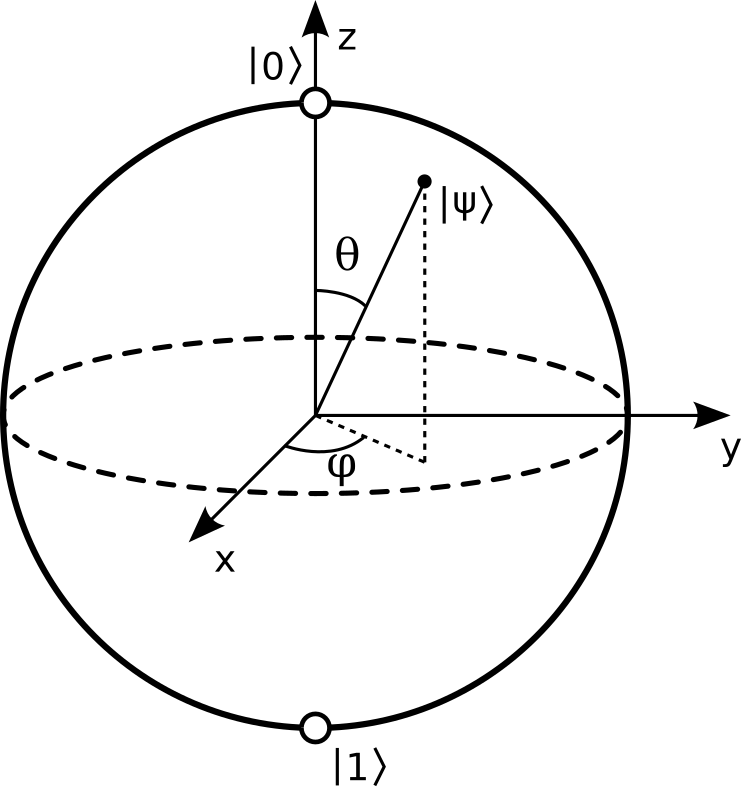
\includegraphics[width=.8\linewidth]{gfx/Bloch_sphere}
    \caption{La sfera di Bloch}
    \label{fig:bloch}
\end{figure}

Gli stati del qubit sull'equatore della sfera, come gli assi coordinati x e y, rappresentano 
sovrapposizioni uniformi dove $\ket{0}$ e $\ket{1}$ hanno entrambi probabilità di misura pari a 
0,5. L'asse x, ad esempio, rappresenta la sovrapposizione uniforme $\frac{1}{\sqrt{2}}
\ket{0} + \frac{1}{\sqrt{2}}\ket{1}$. 
% Come illustrato in Figura, % inserisci riferimento
Qualunque stato bidimensionale arbitrario $\ket{\psi}$ può essere decomposto nei suoi angoli 
polari $\theta$ e $\varphi$ e visualizzato come un vettore sulla sfera di Bloch (dopo essere 
stato normalizzato, se necessario). Tale oggetto è chiamato vettore di Bloch dello stato 
$\ket{\psi}$ del qubit. 

Ad ogni modo, i computer con un solo bit non sono molto utili, e tantomeno i \ac{CQ} con 
un solo qubit. Se prendiamo un byte, ovvero otto bit, possiamo avere una generica 
configurazione 10011101. La rappresentazione associata è 
\begin{equation}
    \ket{1}\otimes\ket{0}\otimes\ket{0}\otimes\ket{1}\otimes\ket{1}\otimes\ket{1}\otimes\ket{0}\otimes\ket{1}.
\end{equation}
Un qubit in questa configurazione appartiene a $\mathbb{C}^2\otimes\mathbb{C}^2\otimes\mathbb{C}^2\otimes\mathbb{C}^2\otimes\mathbb{C}^2\otimes\mathbb{C}^2\otimes\mathbb{C}^2\otimes\mathbb{C}^2 = (\mathbb{C}^2)^{\otimes 8}$. 
Questo spazio vettoriale ha dimensione $2^8=256$. La sua rappresentazione matriciale è allora
\begin{equation}
    \begin{matrix}
        00000000 \\ 
        00000001 \\ 
        \vdots \\ 
        10011101 \\
        \vdots \\
        11111110 \\ 
        11111111
    \end{matrix}
    \begin{pmatrix}
        0 \\ 0 \\ \vdots \\ 1 \\ \vdots \\ 0 \\ 0
    \end{pmatrix}
    .
\end{equation}
La generalizzazione al mondo quantistico è uno stato in sovrapposizione 
\begin{equation}
    \begin{matrix}
        00000000 \\ 
        00000001 \\ 
        \vdots \\
        11111110 \\ 
        11111111
    \end{matrix}
    \begin{pmatrix}
        c_0 \\ c_1 \\ \vdots \\ c_{254} \\ c_{255}
    \end{pmatrix},
\end{equation}
dove $\sum_{i=0}^{255}|c_i|^2=1$. 
Nei computer classici è necessario indicare lo stato di ogni bit in un byte. 
Questo significa scrivere su otto bit. Nel caso quantistico, uno stato di otto 
qubit è dato scrivendo 256 numeri complessi. Questa crescita esponenziale della 
capacità di immagazzinamento dei dati è una delle ragioni per cui i ricercatori 
hanno manifestato interesse per il concetto di quantum computing. 

\subsection{Porte logiche quantistiche} \label{sec:porte_quantistiche}

\begin{definition}
    Una porta logica quantistica è un operatore che agisce sui qubit. Tali operatori 
    saranno rappresentati da matrici unitarie. 
\end{definition}
Le porte logiche quantistiche che agiscono su un sigolo qubit possono essere 
rappresentate come matrici unitarie $2 \times 2$ le cui azioni 
su un qubit possono essere visualizzate come rotazioni o inversioni 
della sfera di Bloch. 

Le porte logiche quantistiche a più qubit agiscono su almeno due qubit 
allo stesso tempo. Similmente alle porte a singolo qubit, una porta quantistica 
a $n$ qubit può essere rappresentata come una matrice unitaria $2^n\times2^n$. 

Tra le porte quantistiche più usate si possono trovare le porte Hadamard, 
NOT, NOT controllata, Toffoli e Fredkin, visibili in figura \ref{fig:porte_1}. 
\begin{figure}[ht!]
    \myfloatalign
    \subfloat[H]{
        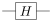
\includegraphics[width=.25\linewidth]{gfx/Hadamard_gate}
    } \quad
    \subfloat[NOT]{
        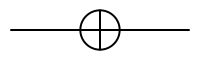
\includegraphics[width=.25\linewidth]{gfx/Qcircuit_NOT}
    } \quad
    \subfloat[cNOT]{
        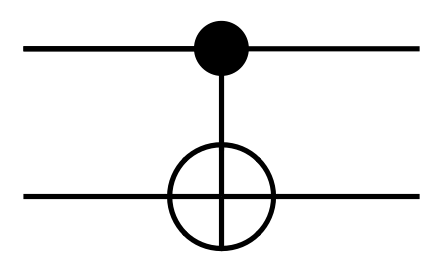
\includegraphics[width=.25\linewidth]{gfx/CNOT_gate}
    } \\ 
    \subfloat[Toffoli]{
        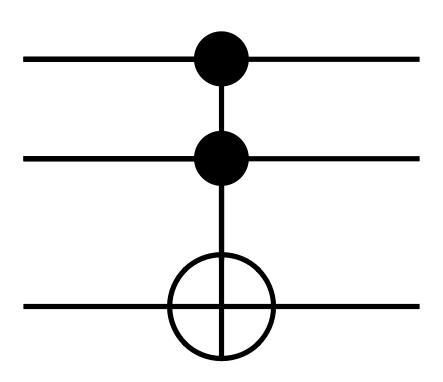
\includegraphics[height=2cm]{gfx/Toffoli_gate}
    } \quad 
    \subfloat[Fredkin]{
        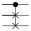
\includegraphics[height=2cm]{gfx/Fredkin_gate}
    }
    
    \caption{Alcune porte quantistiche}
    \label{fig:porte_1}
\end{figure}

Molto importanti sono le tre matrici di Pauli: 
\begin{equation}
    X=\begin{pmatrix}
        0&1\\1&0
    \end{pmatrix},
    \quad Y = \begin{pmatrix}
        0&-1 \\ i&0
    \end{pmatrix},
    \quad Z = \begin{pmatrix}
        1&0 \\ 0&-1
    \end{pmatrix}.
\end{equation}

Altre importanti matrici usate spesso sono 
\begin{equation}
    S=\begin{pmatrix}
        1&0\\0&i
    \end{pmatrix}
    \quad e \quad T = \begin{pmatrix}
        1&0\\0&e^{i\pi/4}
    \end{pmatrix}.
\end{equation}

Le matrici $X$, $Y$ e $Z$ sono modi di girare la 
sfera di Bloch di $\pi$ attorno agli assi $x$, $y$ e $z$ rispettivamente. 
Si noti che $X$ non è altro che la porta NOT, e trasforma $\ket{0}$ in $\ket{1}$ 
e viceversa. Ma per di più porta tutto quello che si trova sopra l'equatore 
sotto di esso. Le altre matrici di Pauli funzionano in maniera simile. 

In alcuni casi non si vuole effettuare una rotazione completa di $\pi$ 
ma si vuole ruotare la sfera di un angolo $\theta$ lungo una particolare direzione. 
In questo caso, dato un vettore tridimensionale $D=(D_x, D_y, D_z)$ di modulo 1, 
possiamo costruire una rotazione della sfera di Bloch attorno ad esso in questo 
modo: 
\begin{equation}
    R_D(\theta)=\cos\frac{\theta}{2}\mathbb{1} - i \sin \frac{\theta}{2} 
    (D_x X + D_y Y + D_z Z). 
\end{equation}

La sfera di Bloch è utile solo per visualizzare stati e trasformazioni di un qubit. 
Quando abbiamo a che fare con più qubit, la dimensionalità degli stati non ci 
permette di avere una rappresentazione intuitivamente semplice. 

Tra le porte a più qubit che verranno usate in questa tesi ci sono le porte controllate: 
queste hanno il loro effetto se tutti i qubit di controllo sono nello stato $\ket{1}$, 
altrimenti lasciano i bersagli della loro azione immutati. 
Si propone a titolo esemplificativo la porta Deutsch, ovvero una rotazione di fase applicata 
a un qubit bersaglio, condizionata dallo stato di due qubit di controllo: 
\begin{equation}
    D_{\theta} : \ket{a,b,c} \mapsto \begin{cases}
        i \cos(\theta)\ket{a,b,c} + \sin(\theta)\ket{a,b,1-c} \quad &\text{per}\, a=b=1, \\ 
        \ket{a,b,c} \quad &\text{altrimenti}.
    \end{cases}
\end{equation}
Nei capitoli successivi verrà implementata la porta $C^n R_y (\theta)$, che effettua una 
rotazione di angolo $\theta$ attorno all'asse y, con $n$ qubit di controllo. 

% *************************************************
% Non si è detto cosa sia un insieme universale di porte
% *************************************************

Le due porte appena descritte non si trovano generalmente nel set universale di porte 
del computer quantistico che si va ad utilizzare, ma devono 
essere approssimate attraverso una successione di porte di base, che può essere più o 
meno lunga. La ricerca di nuovi modi per implementare porte complesse in maniera 
nativa \cite{PhysRevApplied.9.051001} è uno degli sforzi per contrastare il fenomeno della 
decoerenza, uno degli ostacoli sostanziali nel calcolo quantistico. 

\subsection{Decoerenza} \label{sec:decoerenza}

\begin{definition}
    La decoerenza è la perdita di purezza dello stato di un sistema quantistico come risultato 
    di interazione con l'ambiente. 
\end{definition}

Esistono due paramentri per descrivere quanto è stabile un sistema nei confronti della decoerenza \cite{IBM_decoherence}: 
\begin{itemize}
    \item il tempo di decoerenza longitudinale, legato all'emissione energetica, 
    ovvero il decadimento degli stati più energetici verso quelli meno energetici
    (si pensi ad un elettrone nello stato eccitato che decade verso lo stato fondamentale in un atomo);
    \item il tempo di decoerenza trasversale, legato al defasamento, tempo in cui 
    statisticamente uno stato di sovrapposizione decade in una configurazione ben definita. 
\end{itemize}


\section{Machine learning classico} \label{sec:machine_learning}

% ***************************************
% Introduzione al machine learning
% ***************************************

\begin{definition}
    Il machine learning, una branca dell'\ac{IA}, è l'applicazione e lo studio  
    di algoritmi che danno un significato ai dati. 
\end{definition}

Si può dividere la materia in tre tipi principali: l'apprendimento supervisionato, 
l'apprendimento non supervisionato e l'apprendimento per rinforzo. 
Qui si parlerà solo di apprendimento supervisionato. 

L'obiettivo dell'apprendimento supervisionato è di imparare un modello da dati 
etichettati che ci permetta di fare previsioni su dati futuri sconosciuti. 
Con il termine supervisionato si intende l'esistenza di un insieme di campioni 
dove i risultati aspettati (l'appartenenza ad una determinata classe, il 
risultato di una funzione) sono già conosciuti. 

La classificazione
\marginpar{Un esempio di classificatore supervisionato è il filtro contro la posta 
indesiderata, che si può addestrare con un insieme di email già classificate come 
spam o non spam, in modo che esso riconosca in quale categoria vanno le nuove email 
in arrivo.}
è una sottocategoria del machine learning supervisionato il cui 
scopo è di predire le etichette di classe che categorizzano delle nuove istanze, 
basandosi su osservazioni passate. Tali classi sono valori discreti non ordinati 
che possono rappresentare l'appartenenza ad un gruppo delle istanze. 

\subsection{KNN} \label{sec:knn}

Il \acf{KNN} è un algoritmo di machine learning supervisionato per la classificazione. 
È chiamato lazy learner, in quanto non apprende una regola su come discriminare 
le classi dei vettori, ma memorizza il data set di apprendimento tutto intero. 
L'algoritmo in sé è piuttosto semplice e può essere riassunto nei seguenti passaggi: 
\begin{itemize}
    \item scegli il numero $k$ e una metrica per la distanza; 
    \item trova i $k$ elementi più vicini al campione da classificare; 
    \item assegna l'etichetta di classe con un voto a maggioranza. 
\end{itemize}

\begin{figure}[h!]
    \centering
    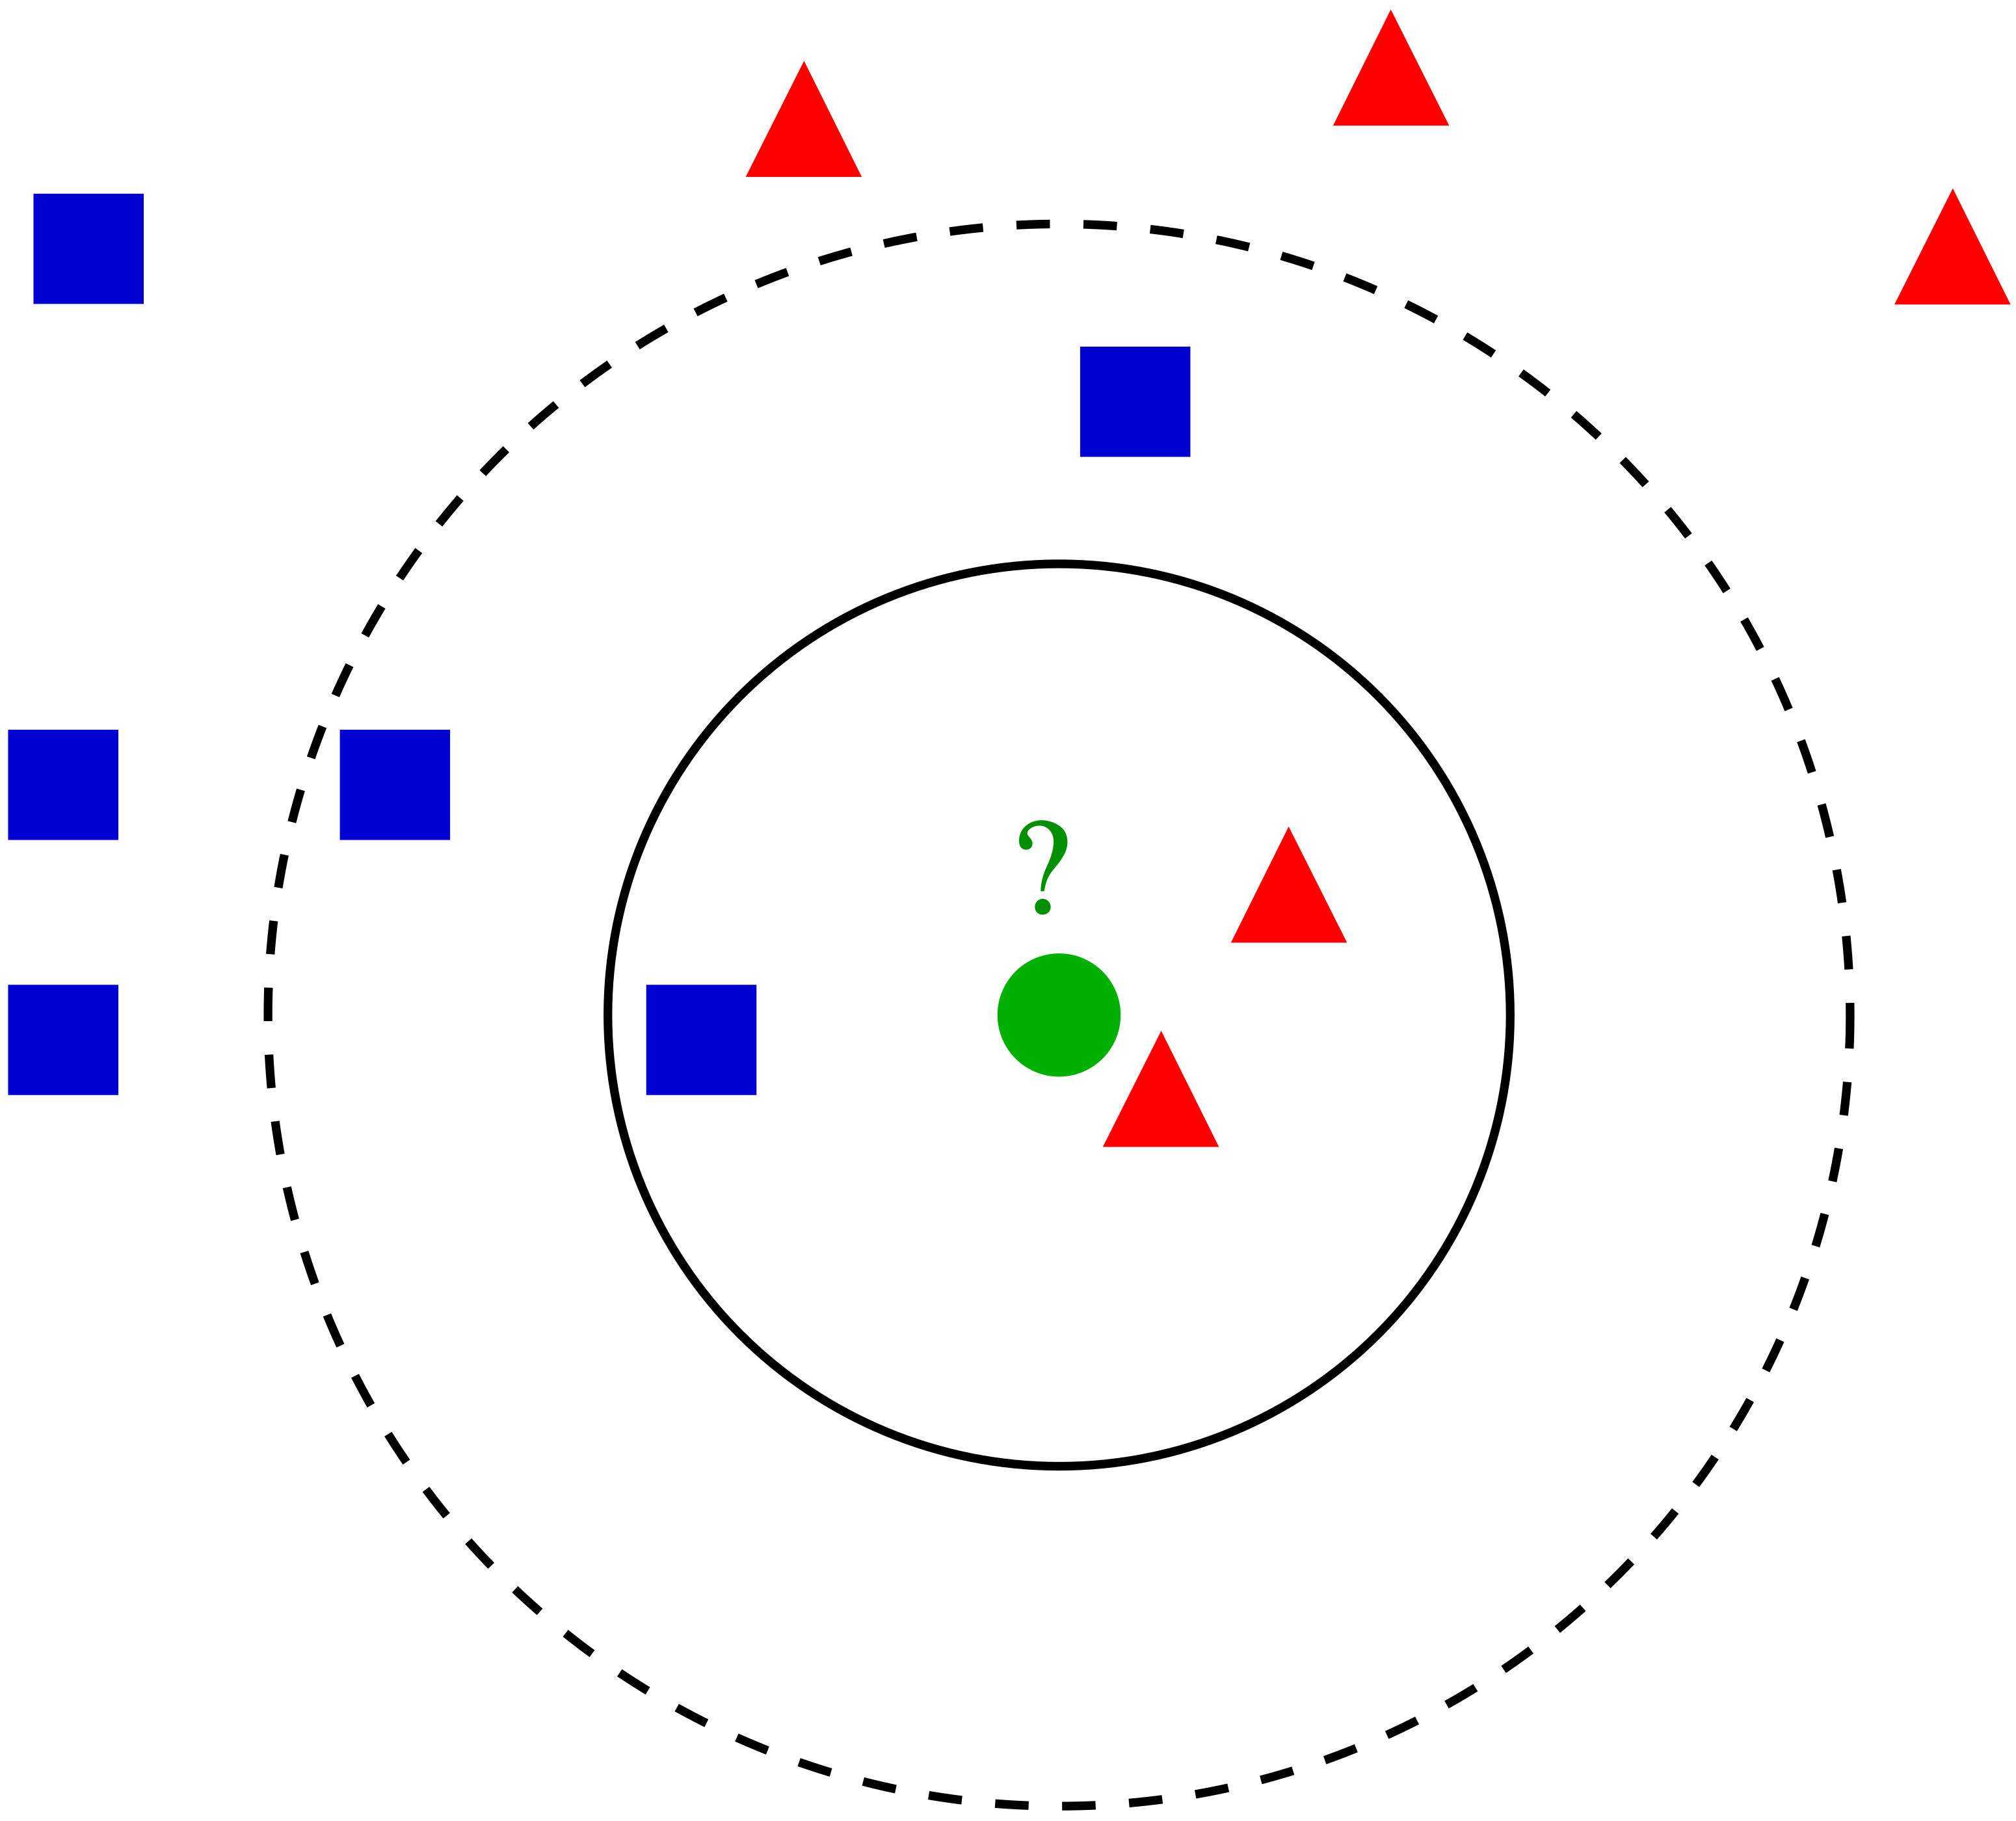
\includegraphics[width=.8\linewidth]{gfx/KnnClassification}
    \caption{Rappresentazione dell'algoritmo \ac{KNN}}
    \label{fig:knn}
\end{figure}

In base alla metrica scelta, l'algoritmo \ac{KNN} trova i $k$ campioni 
nel data set di apprendimento che sono più vicini (simili) al punto 
da classificare. La classe del nuovo punto è allora determinata da un 
voto a maggioranza basato sulla classe a cui appartengono i suoi $k$ 
vicini (vedi figura \ref{fig:knn}). 

Il vantaggio principale di 
questo approccio basato sulla memoria è che il classificatore si 
adatta immediatamente man mano che aggiungiamo vettori di apprendimento. 
Dall'altro lato, il difetto è che la complessità computazionale per 
classificare nuovi campioni cresce al più linearmente con il numero di 
vettori di apprendimento. Per di più, non possiamo ignorare a priori 
alcun vettore di training dato che non c'è un vero e proprio apprendimento. 
Così, lo spazio di archiviazione e il numero di distanze da calcolare possono 
diventare un problema nodale quando si lavora con grandi data set. \cite{pml}

\section{Machine learning quantistico} \label{sec:qml}

% ***************************************
% Introduzione al quantum machine learning, vedi articolo di Biamonte e Lloyd
% ***************************************

% Quantum mechanics is well known to produce atypical patterns in data. Classical machine learning methods such as deep neural networks frequently have the feature that they can both recognize statistical patterns in data and produce data that possess the same statistical patterns: they recognize the patterns that they produce. This observation suggests the following hope. If small quantum information processors can produce statistical patterns that are computationally difficult for a classical computer to produce, then perhaps they can also recognize patterns that are equally difficult to recognize classically.

Il machine learning quantistico è la materia che unisce machine learning e 
meccanica quantistica. Bimonte et al. \cite{Biamonte2017} scrivono: 
% For example, quantum computers can search an unsorted database with N entries in time proportional to √N—that is, O(√N)—where a classical computer given blackbox access to the same database takes time proportional to N: thus the quantum computer exhibits a square-root speedup over the classical computer. Similarly, quantum computers can perform Fourier transforms over N data points, invert sparse N × N matrices, and find their eigenvalues and eigenvectors in time proportional to a polynomial in log2N, where the best known algorithms for classical computers take time proportional to Nlog2N: thus the quantum computer exhibits an exponential speedup over the best classical computer algorithms.
\begin{quote}
    la meccanica quantistica segue notoriamente modelli atipici. 
    I metodi di machine learning classico come le reti neurali profonde 
    (deep neural network) frequentemente hanno la caratteristica di poter sia 
    riconoscere modelli statistici sia produrre dati che ne possiedano gli 
    stessi andamenti: riconoscono i motivi che producono. Questa osservazione 
    porta alla seguente speranza. Se piccoli processori di informazioni 
    quantistiche possono produrre motivi statistici che sono computazionalmente 
    difficili da produrre per un computer classico, allora forse essi possono 
    anche riconoscere motivi che sono ugualmente difficili da riconoscere 
    classicamente. 
    \marginpar{
    Per esempio, i computer quantistici possono cercare in una banca dati non ordinata con 
    $N$ voci in un tempo proporzionale a $\sqrt{N}$, ovvero $\mathcal{O}(\sqrt{N})$, mentre 
    un computer classico con accesso a scatola nera alla stessa banca dati impiega un tempo 
    proporzionale ad $N$: dunque il computer quantistico esibisce un'accelerazione 
    che va come la radice quadrata rispetto al computer classico. 
    }
    La realizzazione di questa speranza dipende dal fatto che si possano trovare algoritmi 
    quantistici efficienti per il machine learning. Un algoritmo quantistico è un insieme di 
    istruzioni che risolvono un problema, come determinare se due grafici sono isomorfi, 
    che possono essere eseguite su un computer quantistico. Il software del quantum machine 
    learning fa uso degli algoritmi quantistici come parte di un'implementazione maggiore. 
    Analizzando i passi prescritti dagli algoritmi quantistici, diventa chiaro che hanno il 
    potenziale di superare in prestazioni gli algoritmi classici per problemi specifici (cioè, 
    ridurre il numero di passi necessari). Questo potenziale è conosciuto come accelerazione 
    quantistica \cite{Ronnow420}. 
\end{quote}
% The realization of this hope depends on whether efficient quantum algorithms can be found for machine learning. A quantum algorithm is a set of instructions solving a problem, such as determining whether two graphs are isomorphic, that can be performed on a quantum computer. Quantum machine learning software makes use of quantum algorithms as part of a larger implementation. By analysing the steps that quantum algorithms prescribe, it becomes clear that they have the potential to outperform classical algorithms for specific problems (that is, reduce the number of steps required). This potential is known as quantum speedup.

Nel quantum machine learning il computer quantistico analizza dati classici, che sono 
codificati come stati quantistici, oppure dati quantistici. Sempre afferente allo stesso 
campo è l'uso di tecniche di machine learning classico per trovare modelli in dinamica 
quantistica. Ci si limiterà al caso dell'uso di computer quantistici per analizzare dati 
classici. 

Nella sezione seguente si descriverà la versione quantistica dell'algoritmo \ac{KNN} visto 
nella sezione \ref{sec:knn}, proposta ed implementata sul processore quantistico a 5 
qubit dell'IBM da Schuld et al. \cite{10.1007/978-3-319-13560-1_17}, \cite{schuld}. 

\subsection{QKNN} \label{sec:qknn}

% ****************************************************
% Desrizione dell'algoritmo di Schuld
% ****************************************************

L'idea alla base dell'algoritmo \ac{QKNN} è di usare il fenomeno di interferenza 
quantistica per ottenere una misura della distanza con un calcolo in parallelo. 
Dotandosi di una procedura efficiente per la preparazione dello stato, l'algoritmo 
ottiene la riduzione logaritmica nelle dimensioni e nel numero di dati in input che 
ci si aspetta usando una codifica quantistica dei dati 
classici \cite{quantum_support_vector_machine}.
Si considera l'attività di classificazione supervisionata di un motivo binario: 
dato un data set $D=\{ (t^1,c^1),\ldots,(t^M,c^M) \}$ di input $t^m\in\mathbb{R}^N$ 
con le rispettive etichette di classe $c^m\in \left\{ -1,1 \right\} $ per $m=1,\ldots,M$ 
e un nuovo input $x\in\mathbb{R}^N$, si trovi l'etichetta $c\in\left\{ -1,1 \right\}$ che 
corrisponde al nuovo input. 

Il classificatore, implementato tramite un circuito di interferenza quantistica 
ed una funzione di soglia, è dato da 
\begin{equation}
    c = \text{sgn} \left( \sum_{m=1}^M c^m \left[ 1 - \frac{1}{4M} | x - t^m |^2 \right] \right). 
\end{equation}
L'algoritmo che implementa il classificatore codifica le caratteristiche dell'input nelle 
ampiezze di probabilità del sistema quantistico e le manipola attraverso porte 
quantistiche; questa strategia è uno dei fattori ritenuti responsabili 
dell'accelerazione quantistica. 
Dato un vettore $x\in\mathbb{R}^N$ normalizzato con modulo unitario e $N=2^n$, 
la codifica nelle ampiezze permette di descrivere lo stato con un registro di $n$ qubit 
$\ket{\psi_x} = \sum_{i=0}^{N-1} x_i \ket{i}$, dove $\ket{i}$ è un registro indice che 
segnala l'$i$-esima componente del vettore classico attraverso l'$i$-esimo elemento della 
base computazionale. 

% La parte sotto è un po' contorta

% L'obiettivo è di classificare una registro di qubit in entrata basandosi 
% su un numero più o meno grande di configurazioni di qubit di apprendimento. 
% Ogni configurazione di apprendimento appartiene ad una certa classe, che è 
% codificata in un registro quantistico di classe in entanglement con la rispettiva 
% configurazione di apprendimento. L'idea principale è che l'algoritmo \ac{KNN} 
% calcola la distanza tra il motivo in entrata ed ogni configurazione di 
% apprendimento attraverso una serie di porte quantistiche. 
% Successivamente, queste distanze sono invertite in modo che i vettori di 
% apprendimento vicini a quello di input hanno l'inverso della distanza 
% maggiore rispetto ai vettori di apprendimento più remoti. Queste distanze inverse 
% sono poi scritte nelle corrispondenti ampiezze dello stato di classe. 
% Si noti che il modulo quadro di un'ampiezza di un particolare stato di classe 
% determina la probabilità di misurare quella classe. 
% Quindi, la probabilità di misurare una data classe dipende adesso dall'inverso 
% delle distanze tra i vettori di apprendimento della classe in esame ed il 
% vettore d'input. L'inverso della distanza può essere visto come un peso 
% dipendente dalla distanza, dato che aumenta la probabilità di misurare la 
% classe con i vettori di apprendimento più vicini a quello d'input. 
% I passaggi necessari per l'implementazione dell'algoritmo \ac{KNN} quantistico 
% sono evidenziati in dettaglio qui di seguito. 

Il primo passo dell'algoritmo consiste nel preparare una 
\emph{sovrapposizione dell'insieme di apprendimento} che 
ne contenga i dati codificati. 
Usando un idoneo schema di preparazione dello stato (nella sezione \ref{sec:ff-qram} 
se ne vedrà un esempio pratico), 
il circuito di classificazione porta un sistema di $n$ 
qubit nello stato 
\begin{equation}
    \ket{D} = \frac{1}{\sqrt{2MC}} \sum_{m=1}^M \ket{m} 
    \left( \ket{0}\ket{\psi_x} + \ket{1}\ket{\psi_{t^m}} \right)
    \ket{c^m}.
\end{equation}
Qui $\ket{m}$ è un registro indice che prende valori 
$m=1,\ldots,M$ e che contrassegna l'$m$-esimo vettore 
di apprendimento. 
Il secondo registro è un singolo qubit ancilla, il cui 
stato eccitato è in entanglement con il terzo registro 
che codifica l'$m$-esimo stato di apprendimento 
$\ket{\psi_{t^m}} = \sum_{i=0}^{N-1} t_i^m \ket{i}$, 
mentre il suo stato fondamentale è in entanglement con 
il terzo registro che codifica il vettore d'input 
$\ket{\psi_x} = \sum_{i=0}^{N-1} x_i \ket{i}$. 
Il quarto registro codifica la classe nell'ampiezza dei propri qubit. 
Effettivamente, si crea una funzione d'onda che contiene 
i vettori di apprendimento insieme ad $M$ copie del nuovo 
input. La costante di normalizzazione $C$ dipende dal 
processo di ottimizzazione dei dati; 
assumeremo in seguito che i vettori di apprendimento siano 
normalizzati e quindi $C=1$. 

Dopo aver preparato lo stato iniziale, il circuito quantistico 
consiste di sole tre operazioni. Prima, l'applicazione di 
una porta Hadamard sull'ancilla fa interferire le copie 
del vettore d'input con i vettori di apprendimento: 
\begin{equation}
    \frac{1}{2\sqrt{M}} \sum_{m=1}^M \ket{m}
    \left( \ket{0}\ket{\psi_{x+t^m}} + \ket{1}  
    \ket{\psi_{x-t^m}} \right) \ket{c^m},
\end{equation}
dove $\ket{\psi_{x \pm t^m}} = \ket{\psi_x} \pm \ket{\psi_{t^m}}$. 

La seconda operazione è una misura condizionale che seleziona 
il ramo con l'ancilla nello stato $\ket{0}$. Questa 
postselezione ha successo con probabilità 
$p_\text{acc} = \frac{1}{4M}\sum_m |x+t^m|^2$. 
È più probabile che abbia successo se la distanza euclidea 
al quadrato complessiva dell'insieme dati di apprendimento 
rispetto al nuovo input è piccola. 
% Mostreremo... ***************
Se la misura condizionale ha successo, lo stato risultanta 
è dato da 
\begin{equation}
    \frac{1}{2\sqrt{Mp_{\text{acc}}}} \sum_{m=1}^M \sum_{i=1}^N 
    \ket{m} ( x_i + t_i^m ) \ket{i} \ket{c^m}.
\end{equation}
Le ampiezze pesano i qubit classe $\ket{c^m}$ con la 
distanza dell'$m$-esimo vettore dati dal nuovo input. 
In questo stato, la probabilità di misurare il qubit 
classe nello stato $\ket{s}$ 
\begin{equation} \label{eq:prob.classe}
    p(\ket{c}=\ket{s}) = \frac{1}{4Mp_{\text{acc}}} 
    \sum_{m|\ket{c}=\ket{s}} |x+t^m|^2,
\end{equation}
riflette la probabilità di predire la classe $s$ per il 
nuovo input. 

La scelta di vettori caratteristica normalizzati assicura che \\ 
$\frac{1}{4Mp_{\text{acc}}}\sum_m |x+t^m|^2 = 
1 - \frac{1}{4Mp_{\text{acc}}}\sum_m |x-t^m|^2$, e la scelta 
della classe con maggior probabilità in questo modo 
implementa il classificatore. 
Questo significa che se il vettore d'input è molto 
vicino ai vettori di training di una data classe, 
quella classe uscirà come risultato più frequentemente 
delle altre. 

% Il \acf{ML}, una sottodisciplina dell'intelligenza artificiale, prova a dare la 
% capacità ai computer di imparare dai dati senza che un umano programmi 
% esplicitamente le sue azioni. Può essere suddiviso nei tre maggiori campi di 
% supervisionato, non supervisionato e apprendimento per rinforzo (Schuld, 
% Sinaskiy, Petruccione, 2015). Solo il machine learning supervisionato sarà 
% introdotto poiché questa tesi di ricerca si focalizza esclusivamente su 
% algoritmi di machine learning supervisionato. 

% L'idea principale del machine learning supervisionato è di addestrare un 
% algoritmo su un insieme di dati \emph{etichettati} contenente, per esempio, 
% immagini di frutti con i corrispondenti nomi cosicché possa essere usato per 
% etichettare nuove immagini che non fanno parte dell'insieme dati di addestramento. 
% Dato che i campioni nell'insieme dati di addestramento sono etichettati, 
% il processo è detto essere supervisionato. 

% Più formalmente, nel machine learning supervisionato si è di fronte a paia di 
% variabili di input (x) e di output (o) e si suppone che l'algoritmo di machine 
% learning impari la funzione $f$ che mappa gli input sui relativi output: 
% \begin{equation} \label{eq:2.38}
%     f(x) = o.
% \end{equation}
% Così, l'algoritmo dovrebbe approssimare la funzione di mappatura $f$ a tal punto 
% che può predire l'output $o$ per nuovi dati di input sconosciuti $\tilde{x}$ 
% (C. M. Bishop, 2006). La seguente sezione introdurrà un algoritmo ben noto nel 
% campo del \ac{ML} supervisionato: l'algoritmo k-nearest neighbours classico. 















% Si immagini di lavorare per una compagnia che gestisce un motore di ricerca e 
% e che venga assegnato il compito di classificare immagini ignote di frutti come 
% mele o banane. Per addestrare l'algoritmo di classificazione, vengono fornite 
% cinque differenti immagini di mele e cinque differenti immagini di banane. 
% Questo verrà chiamato l'\emph{insieme dati di apprendimento} (training data set) 
% $D_T$. Le immagini in $D_T$ potrebbero essere prese da angolazioni diverse, in 
% condizioni di luce varie ed includere mele e banane di colori diversi. 

% La maggior parte delle volte, usare la rappresentazione completa dei pixel di 
% ogni immagine per la classificazione non porta a risultati ottimali. Dunque, il 
% passo successivo è di selezionare un certo numero di caratteristiche (features) 
% estratte dalle immagini nell'insime di apprendimento che possono essere usate per 
% differenziare le mele dalle banane. Tali caratteristiche possono essere il codice 
% del colore più frequente tra i pixel, dato che mele e banane hanno spettri di 
% colore diversi. Usare una misura della curvatura dell'oggetto principale 
% nell'immagine è un'altra possibilità, dato che una mela è quasi sferica mentre 
% una banana assomiglia più ad una linea curva. 

% Selezionando ed estraendo caratteristiche, la dimensionalità dell'insieme dati 
% di apprendimento è drasticamente ridotta da qualche migliaio di pixel ad una 
% manciata di caratteristiche. Le $m$ caratteristiche estratte dalla $j$-esima 
% immagine sono conservate nel $vettore caratteristica$ $m$-dimensionale 
% $\vec{v}_j$. Matematicamente, l'insieme dati di apprendimento $D_T$ consiste di 
% dieci vettori caratteristica $\vec{v}_0, \vec{v}_1, \ldots, \vec{v}_9$, ognuno 
% assegnato alla classe $A$ (mela) o alla classe $B$ (banana). I vettori di 
% apprendimento sono visualizzati come cerchi chiari e scuri in figura. 

% % Metti figura ****************************

% Data una nuova immagine di una mela o una banana, prima si estraggono le stesse 
% $m$ caratteristiche da essa e si conservano nel vettore d'input $\vec{x}$. Dei 
% tanti algoritmi, si sceglie di usare l'algoritmo \ac{KNN}, dato che è un 
% classificatore non parametrico, cioè non fa assunzioni pregresse sulla classe 
% della nuova immagine. Dato un nuovo vettore d'input $\vec{x}$ non classificato 
% (stella nella figura), % inserisci riferimento a figura
% l'algoritmo considera i $k$ elementi più vicini tra quelli dell'insieme dati 
% di apprendimento (usando una misura di distanza predefinita) e classifica 
% $\vec{x}$, basandosi su un voto a maggioranza, come $A$ o $B$. Così, $k$ è un 
% numero intero positivo, solitamente scelto piccolo ed il suo valore determina 
% il risultato della classificazione. Praticamente, nel caso $k=3$ in figura, 
% % aggiungi riferimento a figura ***************
% il vettore $\vec{x}$ sarà classificato come appartenente alla classe $B$ (scuro) 
% ma nel caso $k=6$ sarà etichettato nella classe $A$ (chiaro). 

% % figura classe a classe b ******************

% Nel caso $k=10$, $\vec{x}$ sarà semplicemente assegnato alla classe con più 
% membri. In questo caso, ai vettori di addestramento dovrebbe assegnarsi dei pesi 
% dipendenti dalla distanza (come $\frac{1}{\text{distanza}}$) per aumentare 
% l'influenza dei vettori più vicini al vettore d'input rispetto a quelli più 
% lontani. 











% \subsection{Complessità algoritmica: notazione O-grande}

% Nei campi dell'informatica e della quantum information, la cosiddetta 
% \emph{notazione O-grande}, inizialmente descritta da Bachmann (1894), 
% % inserisci fonte *****************************
% è spesso usata per descrivere come l'esecuzione di un algoritmo dipende 
% da variabili come l'accuratezza desiderata, il numero di vettori d'input o la 
% loro dimensione. Per questo, essa è un modo di quantificare la \emph{complessità 
% in termini di tempo dell'algoritmo} di un algoritmo quantistico. Nelle sezioni 
% successive di questa tesi, la notazione O-grande sarà usata come uno strumento 
% per quantificare possibili accelerazioni quantistiche negli algoritmi \ac{KNN} di 
% machine learning quantistico. 

% % scatola definizione di big-O **************

% % continuare ********************




% Un buon esempio di un'implementazione fisica di un qubit è il singolo elettrone di un atomo di 
% idrogeno abbozzato in figura. % metti riferimento a figura
% Solitamente l'elettrone si trova % è trovato
% nel suo stato fondamentale, che può essere definito come lo stato $\ket{0}$ del qubit. 
% Usando un impulso laser, l'elettrone può essere eccitato verso il guscio di valenza successivo più 
% energetico, che può essere definito come lo stato $\ket{1}$  del qubit. Dopo del tempo $t$ 
% l'elettrone decadrà per decoerenza verso il suo stato fondamentale $\ket{0}$; questo tempo è 
% chiamato \emph{tempo di decoerenza longitudinale} o \emph{di smorzamento dell'ampiezza} ed è 
% un parametro importante per misurare la vita dei qubit. % Fonte Chuang, 2003

% Figura ***********************************

% Un bit classico non probabilistico può assumere solo uno dei suoi due possibili valori alla volta. 
% Qui si potrebbe mettere una nota sui bit probabilistici
% Al contrario, i qubit obbediscono alle leggi della meccanica quantistica, il che dà luogo 
% all'importante proprietà che, oltre ad essere in un definito stato $\ket{0}$ o $\ket{1}$, 
% possono anche essere in una sovrapposizione di due stati. Matematicamente ciò è espresso 
% attraverso la combinazione lineare degli stati $\ket{0}$ e $\ket{1}$
% \begin{equation} \label{eq:2.1}
%     \ket{\psi} = \alpha \ket{0} + \beta \ket{1}, \quad \alpha, \beta \in \mathbb{C},
% \end{equation}
% dove $\alpha$ e $\beta$ sono coefficienti complessi e ci si riferisce spesso a loro come ampiezze. 
% Qualsiasi ampiezza $\eta$ può essere ulteriormente suddivisa in un fattore di fase complesso 
% $e^{i\varphi}$ ed un numero reale non negativo $\xi$ cosicché
% \begin{equation}
%     \eta = e^{i\varphi} \xi.
% \end{equation}
% Nella prima equazione, $\ket{0}$ è la rappresentazione nella notazione di Dirac del fatto che il 
% qubit sia nello stato 0 e può essere rappresentato come un elemento di uno spazio vettoriale 
% complesso bidimensionale $H_2$, % metti il font giusto ad H
% detto spazio di Hilbert. Inizialmente definito da Dirac, % metti fonte 1939
% l'oggetto 
% \begin{equation}
%     \ket{\varphi},
% \end{equation}
% è chiamato \emph{ket} e il suo coniugato hermitiano 
% \begin{equation}
%     \ket{\varphi}^\dagger = \bra{\varphi}
% \end{equation}
% è chiamato \emph{bra}. Il coniugato hermitiano, denotato con una daga ($\dagger$), di p.e. un 
% vettore colonna $c$ bidimensionale a valori complessi $c_1$ e $c_2$, 
% \begin{equation}
%     c = 
%     \begin{pmatrix}
%         c_1\\c_2
%     \end{pmatrix},
% \end{equation}
% è ottenuto prendendo il complesso coniugato di ciascun valore e trasponendo il vettore risultante: 
% \begin{equation}
%     c^\dagger = 
%     \begin{pmatrix}
%         c_1\\c_2
%     \end{pmatrix}^\dagger
%     = 
%     \begin{pmatrix}
%         c_1^* & c_2^*
%     \end{pmatrix},
% \end{equation}
% dove i complessi coniugati sono indicati con un asterisco in apice ($*$).
% Il coniugato hermitiano è definito sia per vettori che per matrici quadrate. 
% Il prodotto interno tra un bra e un ket è chiamato \emph{bra-ket} ed è scritto 
% \begin{equation}
%     \braket{\varphi|\varphi}.
% \end{equation}
% Si noti che tutte le sezioni seguenti faranno uso intensivo della notazione bra-ket. 
% Gli stati quantistici $\ket{0}$ e $\ket{1}$ sono chiamati la base computazionale e 
% costituiscono una base ortonormale di $H_2$. Quando un qubit è espresso in termini 
% dei due stati $\ket{0}$ e $\ket{1}$, si dice che sia nella sua \emph{base normale}. 
% Per motivi di chiarezza, $\ket{0}$ e $\ket{1}$ possono essere rappresentati con i vettori 
% bidimensionali 
% \begin{equation} \label{eq:2.8}
%     \ket{0} \cong \begin{pmatrix}
%         1\\0
%     \end{pmatrix}
%     \text{e} \ket{1} \cong \begin{pmatrix}
%         0\\1
%     \end{pmatrix}.
% \end{equation}
% Si noti che un ket e la sua rappresentazione vettoriale non sono lo stesso oggetto, 
% dato che, per essere ben definito, un vettore ha bisogno della specificazione di una base, 
% laddove un ket non lo richiede. Questa tesi farà uso del simbolo $\cong$ quando si cambia tra 
% i due diversi modi di rappresentare un ket. Sostituendo i vettori dell'Eq. \ref{eq:2.8} 
% nell'Eq. \ref{eq:2.1} si ottiene la rappresentazione vettoriale di $\ket{\psi}$
% \begin{equation} \label{eq:2.9}
%     \psi \cong \alpha \begin{pmatrix}
%         1\\0
%     \end{pmatrix} + \beta \begin{pmatrix}
%         0\\1
%     \end{pmatrix} = \begin{pmatrix}
%         \alpha \\ \beta
%     \end{pmatrix}.
% \end{equation}

% Sebbene un qubit possa essere in una sovrapposizione di stati $\ket{0}$ e $\ket{1}$, quando 
% misurato assumerà un valore preciso tra $\ket{0}$, con probabilità 
% \begin{equation}
%     P(\ket{0}) = |\alpha|^2,
% \end{equation}
% e $\ket{1}$, con probabilità 
% \begin{equation}
%     P(\ket{1}) = |\beta|^2.
% \end{equation}
% Il fatto che la probabilità di misurare un particolare stato è uguale al quadrato del modulo 
% della rispettiva ampiezza fu postulato per la prima volta da Born % Fonte 1954
% e, dunque, è chiamata regola di Born. Visto che la probabilità totale di misurare un qualunque 
% valore deve essere unitaria, deve soddisfarsi la condizione di normalizzazione 
% \begin{equation}
%     |\alpha|^2 + |\beta|^2 = 1.
% \end{equation}

% Se prendiamo uno stato in cui si ha, per esempio, $\alpha = \frac{1}{\sqrt{2}}$ e 
% $\beta = \frac{i}{\sqrt{2}}$, abbiamo che il qubit è in una sovrapposizione quantistica, 
% cosa impossibile da ottenere con un computer classico. Legato a questa caratteristica 
% c'è un altro importante parametro della vita di un qubit: il \emph{tempo di coerenza 
% trasversale} o \emph{di smorzamento della fase}. 
% Esso è misurato preparando la sovrapposizione uniforme $\frac{\ket{0} + \ket{1}}{\sqrt{2}}$: 
% per via dell'inevitabile interazione con l'ambiente, dopo del tempo $t$ il comportamento 
% quantistico sarà perso e lo stato sarà ben determinato tra $\ket{0}$ e $\ket{1}$. % Fonte Chuang 2003
% Il processo di perdita del comportamento quantistico è chiamato decoerenza. 
% Nei casi in cui $\alpha = 1$ o $\beta = 1$ il qubit non è propriamente in una sovrapposizione ma 
% in uno stato definito, $\ket{0}$ o $\ket{1}$ rispettivamente. 

% Perciò, un qubit è intrinsecamente probabilistico ma quando viene misurato collassa in un 
% singolo bit classico (0 o 1). 
% % Da qualche parte si può inserire un riferimento alla probabilità negativa riferita sul Noson
% Ne segue che una misura distrugge l'informazione sulla sovrapposizione del qubit (ovvero i valori 
% di $\alpha$ e $\beta$). Questo costituisce una delle principali difficoltà nel progettare 
% algoritmi quantistici, dato che solo una limitata quantità di informazioni può essere ottenuta 
% riguardo gli stati finali dei qubit nel computer quantistico. 

%%% Figura

% Didascalia della figura

% Similmente alle porte logiche in un computer classico, un \ac{CQ} manipola qubit per mezzo di porte 
% logiche quantistiche, le quali saranno introdotte in dettaglio nella sezione 2.2. In genere, 
% una porta logica quantistica arbitraria $U$ che agisca su uno stato di singolo qubit è una 
% trasformazione unitaria che può essere rappresentata con una matrice 2x2
% \begin{equation} \label{eq:2.14}
%     U \cong 
%     \begin{pmatrix}
%         a & b \\ c & d
%     \end{pmatrix},
% \end{equation}
% la cui azione su $\ket{\psi}$ è definita come 
% \begin{equation}
%     U\ket{\psi} \cong \begin{pmatrix}
%         a&b\\c&d
%     \end{pmatrix}\begin{pmatrix}
%         \alpha\\\beta
%     \end{pmatrix} = \begin{pmatrix}
%         a\alpha + b\beta \\ c\alpha + d\beta
%     \end{pmatrix}.
% \end{equation}
% La matrice $U$ deve essere unitaria, il che comporta che il suo determinante deve essere unitario: 
% \begin{equation}
%     |\det(U)|=1,
% \end{equation}
% e il suo coniugato hermitiano $U^\dagger$ deve essere uguale alla sua inversa: 
% \begin{equation}
%     UU^\dagger = U^\dagger U = \mathbb{1} = UU^{-1} = U^{-1}U.
% \end{equation}
% Tutte le porte logiche quantistiche devono essere unitarie poiché in questo modo si conserva 
% la condizione di normalizzazione dello stato del qubit su cui agiscono. L'insieme di tutte 
% le matrici complesse unitarie bidimensionali con determinante uguale ad uno è chiamato gruppo 
% unitario speciale ($SU(2)$) e tutte le porte logiche quantistiche a singolo qubit sono dunque 
% elementi di $SU(2)$. Inoltre, un insieme di porte $G$ costituito da $m$ porte quantistiche 
% $g_1, g_2, \ldots, g_m$ è chiamato \emph{insieme di porte quantistiche universale} allorquando 
% è un sottoinsieme denso di $SU(2)$ come definito nel riquadro seguente.

% Definizione: sottoinsieme denso di $SU(2)$

% L'insieme di porte $G$ è un sottoinsieme denso di $SU(2)$ quanto, data una qualunque porta 
% quantistica $W\in SU(2)$ e una precisione arbitraria $\varepsilon > 0$, esiste un prodotto 
% $J$ di porte appartenenti a $G$ che è una $\varepsilon$-approssimazione di $W$ 
% (Dawson, Nielsen, 2005). 
















% \subsection{Sistemi a qubit multipli}

% Un computer classico coun un bit di memoria non è particolarmente utile e, allo stesso modo, 
% un \ac{CQ} con un qubit è piuttosto inutile. Per essere in grado di effettuare computazioni 
% grandi e complicate è necessario combinare diversi qubit singoli per creare un grande \ac{CQ}. 
% Quando ci si muove da un sistema a singolo qubit ad uno a molti qubit c'è bisogno di un 
% nuovo strumento matematico, il cosiddetto prodotto tensoriale (simbolo $\otimes$). 
% Il prodotto tensore di due qubit si scrive 
% \begin{equation} \label{eq:2.18}
%     \ket{\psi_1}\otimes\ket{\psi_2} = \ket{\psi_1}\ket{\psi_2} = \ket{\psi_1\psi_2},
% \end{equation}
% dove nelle ultime due espressioni si è omesso il simbolo $\otimes$; queste due sono 
% una stenografia per il prodotto tensore tra due qubit. 

% Un \emph{registro quantistico} di dimensione $j$ è una maniera alternativa di riferirsi 
% al prodotto tensore di $j$ qubit. Per esempio, lo stato nell'Eq. \ref{eq:2.18} è un 
% registro quantistico composto da due qubit. Negli algoritmi di \ac{MLQ}, grandi stati 
% quantistici sono solitamente suddivisi in vari registri quantistici che soddisfano vari 
% obiettivi, p.e. memorizzare etichette di dati o di classi. Si consideri, ad esempio, uno 
% stato quantistico $\ket{\Phi}$ che sia suddiviso tra due diversi registri quantistici, 
% un registro dati (d) con $n$ qubit e un registro classe (c) con due qubit. Lo stato $\ket{\Phi}$ 
% si scrive allora 
% \begin{equation} \label{eq:2.19}
%     \ket{\Phi} = \ket{d;c} = \ket{d_1 \ldots d_n; c_1, c_2},
% \end{equation}
% dove i punti e virgola sono usati per separare i registri quantistici. 

% Nella rappresentazione vettoriale, il prodotto tensore di due ket $\ket{0}$ è definito come 
% \begin{equation} \label{eq:2.20}
%     \ket{00} = \ket{0} \otimes \ket{0} \cong 
%     \begin{pmatrix}
%         1\\0
%     \end{pmatrix} \otimes 
%     \begin{pmatrix}
%         1\\0
%     \end{pmatrix} = 
%     \begin{pmatrix}
%         1*\begin{pmatrix}
%             1\\0
%         \end{pmatrix} \\ 0 * 
%         \begin{pmatrix}
%             1\\0
%         \end{pmatrix}
%     \end{pmatrix} = 
%     \begin{pmatrix}
%         1\\0\\0\\0
%     \end{pmatrix}.
% \end{equation}
% L'ultima espressione nell'Eq. \ref{eq:2.20} mostra che lo stato a due qubit $\ket{00}$ non è 
% più bidimensionale ma quadridimensionale. Dunque, vive in uno spazio di Hilbert quadridimensionale 
% $\mathcal{H}_4$. Una porta quantistica che agisca su molti qubit può allora non avere le stesse 
% dimensioni di una porta a singolo qubit (Eq. \ref{eq:2.14}), il che richiede un nuovo formalismo 
% per le porte per sistemi a qubit multipli. 

% Si provi ad applicare un'arbitraria porta a singolo qubit U (Eq. \ref{eq:2.14}) 
% al primo qubit nello stato a due qubit $\ket{00}$. Il secondo qubit dello stato 
% $\ket{00}$ dovrebbe rimanere immutato, che, in altre parole, significa applicare 
% la matrice identità $\mathbb{1}$ 2x2 su di esso. Per effettuare queste operazioni, 
% si definisce il prodotto tensore delle due porte a singolo qubit come 
% \begin{equation}
%     \begin{split}
%     &U\otimes\mathbb{1}\cong
%     \begin{pmatrix}
%         a&b\\c&d
%     \end{pmatrix}
%     \otimes
%     \begin{pmatrix}
%         1&0\\0&1
%     \end{pmatrix} = \\
%     &=
%     \begin{pmatrix}
%         a*
%         \begin{pmatrix}
%             1&0\\0&1
%         \end{pmatrix}
%         &b*
%         \begin{pmatrix}
%             1&0\\0&1
%         \end{pmatrix}
%         \\c*
%         \begin{pmatrix}
%             1&0\\0&1
%         \end{pmatrix}
%         &d*
%         \begin{pmatrix}
%             1&0\\0&1
%         \end{pmatrix}
%     \end{pmatrix}
%     =
%     \begin{pmatrix}
%         a&0&b&0\\
%         0&a&0&b\\
%         c&0&d&0\\
%         0&c&0&d
%     \end{pmatrix}.
%     \end{split}
% \end{equation} % vedi come andare a capo nelle equazioni
% Dunque, il risultato del prodotto tensore $U\otimes\mathbb{1}$ può essere 
% rappresentato come una matrice unitaria 4x4 che può ora essere usata per 
% trasformare il vettore 4x1 che rappresenta lo stato $\ket{00}$ nell'Eq. \ref{eq:2.20}: 
% \begin{equation} \label{eq:2.22}
%     U\otimes\mathbb{1}\ket{00}\cong
%     \begin{pmatrix}
%         a&0&b&0\\
%         0&a&0&b\\
%         c&0&d&0\\
%         0&c&0&d
%     \end{pmatrix}
%     \begin{pmatrix}
%         1\\0\\0\\0
%     \end{pmatrix}
%     =
%     \begin{pmatrix}
%         a\\0\\c\\0
%     \end{pmatrix}
%     .
% \end{equation}
% Si può anche effettuare prima le operazioni di singolo qubit sui rispettivi 
% qubit, seguite dal prodotto tensore dei due risultanti vettori: 
% \begin{equation} \label{eq:2.23}
%     \begin{split}
%     &(U\otimes\mathbb{1})(\ket{0}\otimes\ket{0}) = 
%     U\ket{0}\otimes\mathbb{1}\ket{0} \cong \\
%     &\cong
%     \begin{pmatrix}
%         a&b\\c&d
%     \end{pmatrix}
%     \begin{pmatrix}
%         1\\0
%     \end{pmatrix}
%     \otimes\Id
%     \begin{pmatrix}
%         1\\0
%     \end{pmatrix}
%     = 
%     \begin{pmatrix}
%         a\\c
%     \end{pmatrix}
%     \otimes
%     \begin{pmatrix}
%         1\\0
%     \end{pmatrix}
%     = 
%     \begin{pmatrix}
%         a\\0\\c\\0
%     \end{pmatrix}
%     .
%     \end{split}
% \end{equation}
% Questo formalismo può essere esteso a qualunque numero di qubit, e l'uso 
% del prodotto tensore porta ad un aumento esponenziale della dimensionalità 
% dello spazio di Hilbert. Così, $n$ qubit vivono in uno spazio di Hilbert 
% $2^n$-dimensionale ($\mathcal{H}_2^{\otimes n}$) e possono immagazzinare 
% il contenuto di $2^n$ bit classici. Per fare un esempio, solo 33 qubit 
% possono contenere l'equivalente di $2^33 = 8589934592$ bit % verificare
% (= 1 gigabyte), il che porta chiaramente con sè il potenziale per le 
% enormi accelerazioni nella potenza di calcolo, come verrà mostrato più avanti. 

% Quando si considerano sistemi a molti qubit, si incontreranno stati quantistici 
% che possono o meno essere fattorizzati. Per esempio, si provi a riscrivere 
% l'ultima espressione dell'Eq. \ref{eq:2.23} come 
% \begin{equation} \label{eq:2.24}
%     \begin{pmatrix}
%         a\\0\\c\\0
%     \end{pmatrix}
%     = a 
%     \begin{pmatrix}
%         1\\0\\0\\0
%     \end{pmatrix}
%     + 0 
%     \begin{pmatrix}
%         0\\1\\0\\0
%     \end{pmatrix}
%     + c 
%     \begin{pmatrix}
%         0\\0\\1\\0
%     \end{pmatrix}
%     + 0 
%     \begin{pmatrix}
%         0\\0\\0\\1
%     \end{pmatrix}
%     \cong a \ket{00} + c \ket{10}, 
% \end{equation}
% che può essere fattorizzato nel prodotto tensore 
% \begin{equation} \label{eq:2.25}
%     a \ket{00} + c \ket{10} = (a \ket{0} + c \ket{1}) \otimes \ket{0}.
% \end{equation}
% Al contrario, si consideri uno dei quattro famosi stati di Bell: 
% \begin{equation} \label{eq:2.26}
%     \ket{\psi^+} = \frac{\ket{01}+\ket{10}}{\sqrt{2}}.
% \end{equation}
% È semplice verificare che lo stato a due qubit $\ket{\psi^+}$ non può essere 
% fattorizzato in un prodotto tensore di due stati di singolo qubit. Ora si 
% immagini che a due persone, Allegra e Bernardo, vengano dati due elettroni 
% preparati nello stato quantistico $\ket{\psi^+}$. Allegra tiene il primo 
% elettrone nel laboratorio e Bernardo porta il secondo elettrone a casa sua. 
% Dopo del tempo $t$, Allegra diventa curiosa di misurare se il suo elettrone 
% è nello stato $\ket{0}$ o $\ket{1}$ ed effettua una misura lungo la base 
% normale. Applicando la regola di Born allo stato quantistico $\ket{\psi^+}$, 
% Allegra sa che misurerà il suo elettrone in uno tra gli stati $\ket{0}$ e 
% $\ket{1}$ con uguali probabilità 0,5. Si noti che, sebbene il vettore di stato 
% $\ket{\psi^+}$ sia conosciuto con esattezza, il risultato della misura è 
% ancora incerto. Misurando il suo elettrone lo trova essere nel suo stato 
% $\ket{1}$. A partire dall'Eq. \ref{eq:2.26}, sapendo che la misura fa 
% collassare una sovrapposizione, lo stato post misura (PM) % definire acronimo?
% $\ket{\psi^+}_{PM}$ è 
% \begin{equation} \label{eq:2.27}
%     \ket{\psi^+}_{PM} = \ket{1_A 0_B}, 
% \end{equation}
% dove i pedici indicano quale elettrone appartiene ad Allegra (A) e quale a 
% Bernardo (B). Osservando questa espressione, Allegra sa che l'elettrone di 
% Bernardo deve trovarsi nello stato $\ket{0}$ senza aver misurato il secondo 
% elettrone! A casa sua, Bernardo misura il suo elettrone un secondo dopo che 
% Allegra ha effettuato la sua misura e trova che infatti è nello stato $\ket{0}$. 
% Si noti che il secondo elettrone non era per niente vicino ad Allegra ma è stata 
% lo stesso in grado di determinare lo stato del secondo elettrone solo misurando 
% il suo. Dopo aver ripetuto questo esperimento un migliaio di volte, Allegra e 
% Bernardo trovano perfette correlazioni nei loro risultati: ogni volta che Allegra 
% misurava il suo elettrone nello stato $\ket{0}$, Bernardo trovava il suo nello 
% stato $\ket{1}$ e viceversa. 

% Le correlazioni non locali tra i risultati di misura di qubit sono una peculiare 
% proprietà quantistica degli stati quantistici non fattorizzabili ed è chiamata 
% \emph{entanglement quantistico} (entanglement significa groviglio, garbuglio 
% in inglese). 
% % Il Vocabolario Garzanti Hazon di Inglese, Garzanti Linguistica, 2010
% % Significa anche coinvolgimento (sentimentale) e forse è per questo che ci sono 
% % tante storie romantiche basate sull'entanglement. 
% È una parte integrante della calcolo quantistico e la sezione 2.2.2 darà un 
% esempio concreto di come creare uno stato in entanglement in un \ac{CQ}. 

% Fino a questo punto, la maggior parte dei concetti introdotti viene dal campo 
% della teoria quantistica pura. Ad ogni modo, questa sezione segna la fondamentale 
% transizione dal campo della teoria quantistica a quello dell'\emph{elaborazione 
% dell'informazione quantistica} (quantum information processing). Un computer 
% classico elabora l'informazione ed effettua calcoli manipolando sistematicamente 
% bit attraverso l'applicazione di porte logiche come le porte NOT o XOR. 
% Analogamente, un computer quantistico elabora l'informazione ed effettua 
% \emph{calcoli quantistici} manipolando qubit usando \emph{porte logiche 
% quantistiche}, spesso chiamate semplicemente \emph{porte quantistiche}. 
% Solitamente, una sequenza di tali porte quantistiche è richiesta per effettuare 
% un certo compito o per risolvere un particolare problema su un computer 
% quantistico. Tale sequenza di porte quantistiche è chiamata \emph{algoritmo 
% quantistico}. 

% Ci sono molti modi diversi di realizzare un \ac{CQ}, per esempio usando ioni 
% intrappolati, fotoni o giunzioni Josephson superconduttive. % Fonti
% A seconda del substrato scelto, possono essere implementati diversi insiemi di 
% porte logiche quantistiche e per eseguire un algoritmo quantistico questo deve 
% essere mappato sull'hardware quantistico disponibile. Dunque, gli algoritmi 
% quantistici hanno bisogno di essere tradotti (compilati) in una serie di porte 
% consistenti solo di porte quantistiche dall'insieme universale di porte 
% disponibile. Ci si riferisce a questo procedimento con \emph{compilazione 
% quantistica}. Le sottosezioni seguenti introdurranno alcune porte logiche 
% quantistiche principali a singolo qubit e multipli qubit che saranno usate 
% estensivamente nelle sezioni successive di questa tesi. 








% \subsection{Porte a singolo qubit}











% Come una porta quantistica a singolo qubit agisca su un qubit, le sue 
% proprietà e rappresentazione matriciale sranno illustrate usando l'esempio 
% dell'equivalente quantistico della porta logica NOT classica: la cosiddetta 
% porta X. La porta X può essere rappresentata dalla matrice unitaria 2x2 
% \begin{equation} \label{eq:2.28}
%     X \cong 
%     \begin{pmatrix}
%         0&1\\1&0
%     \end{pmatrix}
%     .
% \end{equation}
% L'azione della porta X sullo stato di qubit arbitrario $\ket{\psi}$ 
% (Eq. \ref{eq:2.9}) può essere analizzata usando la matrice della porta e la 
% rappresentazione vettoriale del qubit. Applicando della semplice algebra lineare 
% si ottiene 
% \begin{equation} \label{eq:2.29}
%     X \ket{\psi} = X (\alpha \ket{0} + \beta \ket{1}) \cong 
%     \begin{pmatrix}
%         0&1\\1&0
%     \end{pmatrix}
%     \begin{pmatrix}
%         \alpha \\ \beta
%     \end{pmatrix}
%     = 
%     \begin{pmatrix}
%         \beta \\ \alpha
%     \end{pmatrix}
%     \cong \beta \ket{0} + \alpha \ket{1}.
% \end{equation}

% Così, applicando la porta X allo stato di qubit $\ket{\psi}$ si scambiano le 
% ampiezze degli stati $\ket{0}$ e $\ket{1}$. Più nello specifico, l'applicazione 
% di X allo stato $\ket{0}$ risulta nello stato $\ket{1}$: 
% \begin{equation} \label{eq:2.30}
%     X \ket{0} \cong 
%     \begin{pmatrix}
%         0&1\\1&0
%     \end{pmatrix}
%     \begin{pmatrix}
%         1\\0
%     \end{pmatrix}
%     =
%     \begin{pmatrix}
%         0\\1
%     \end{pmatrix}
%     \cong \ket{1}.
% \end{equation}
% Nei termini dell'esempio con l'elettrone di valenza di un atomo di idrogeno 
% mostrato in Fig. 2.1, una porta X può essere implementata eccitando l'elettrone 
% dallo stato fondamentale $\ket{0}$ verso il guscio di valenza successivo più 
% energetico dell'elettrone, definito come stato $\ket{1}$, usando un impulso 
% laser controllato. 

% Lo stato $\ket{0}$ è recuperato quando si applica di nuovo X allo stato $\ket{1}$: 
% \begin{equation} \label{eq:2.31}
%     X \ket{1} \cong 
%     \begin{pmatrix}
%         0&1\\1&0
%     \end{pmatrix}
%     \begin{pmatrix}
%         0\\1
%     \end{pmatrix}
%     = 
%     \begin{pmatrix}
%         1\\0
%     \end{pmatrix}
%     \cong \ket{0}.
% \end{equation}
% Sulla sfera di Bloch, la porta X corrisponde ad una rotazione antioraria di $\pi$ 
% attorno all'asse x, come mostrato in Fig. 2.3.

% % Figura ***********************

% Dalle Eq. \ref{eq:2.29}, \ref{eq:2.30} e \ref{eq:2.31} segue che X è la propria 
% inversa così come il proprio coniugato hermitiano: 
% \begin{equation} \label{eq:2.32}
%     XX = XX^\dagger = \mathbb{1},
% \end{equation}
% \begin{equation} \label{eq:2.33}
%     X = X^{-1} = X^\dagger.
% \end{equation}
% Basandosi sul libro di testo di Nielsen e Chuang (2010), % inserisci fonte
% l'azione, la rappresentazione del circuito e della matrice e la visualizzazione 
% sulla sfera di Bloch per alcune delle più importanti porte logiche quantistiche 
% a singolo qubit sono riassunte nella tabella 2.1.

% % tabella ***************************************












% \subsection{Porte a qubit multipli}












% % Tabella **********************

% La porta quantistica NOT controllata a due qubit 
% sarà usata per dimostrare le proprietà, la rappresentazione matriciale e l'azione 
% di una porta quantistica a due qubit. Questo può poi essere facilmente 
% generalizzato a porte quantistiche a $n$ qubit. 

% La porta NOT controllata o CNOT è data dalla seguente matrice $4\times4$: 
% \begin{equation} \label{eq:2.34}
%     \text{CNOT} \cong 
%     \begin{pmatrix}
%         \mathbb{1} & 0 \\ 0 & X
%     \end{pmatrix}
%     =
%     \begin{pmatrix}
%         1&0&0&0\\
%         0&1&0&0\\
%         0&0&0&1\\
%         0&0&1&0
%     \end{pmatrix}
%     .
% \end{equation}
% La porta CNOT accetta due qubit, uno di controllo e uno bersaglio, come input. 
% Se e solo se il qubit di controllo è nello stato $\ket{1}$, la porta quantistica 
% NOT (X) è applicata al qubit bersaglio. Nelle equazioni, la CNOT sarà sempre 
% seguita da parentesi contenenti il qubit di controllo (c) seguito dal qubit 
% bersaglio (b): % oppure usare t come lettera
% CNOT(c,b). La relazione di input-output, chiamata tabella di verità, per la porta 
% CNOT è data nella tabella 2.2. 

% Per dimostrare l'utilità della porta CNOT si immagini di iniziare con due 
% qubit non in entanglement, entrambi nello stato $\ket{0}$: 
% \begin{equation} \label{eq:2.35}
%     \ket{\varphi_0} = \ket{0} \otimes \ket{0} = \ket{00}.
% \end{equation}
% Applicando la porta H sul primo qubit si ottiene il seguente stato (ancora non 
% in entanglement): 
% \begin{equation} \label{eq:2.36}
%     \ket{\varphi_1} = (H \otimes \mathbb{1}) \ket{\varphi_0} = 
%     (H \otimes \mathbb{1}) \ket{00} = \frac{1}{\sqrt{2}} \ket{00} + 
%     \frac{1}{\sqrt{2}} \ket{10}.
% \end{equation}
% Ora si immagini di applicare la porta CNOT allo stato $\ket{\varphi_1}$, in cui 
% il qubit di controllo è quello di sinistra e il qubit bersaglio è quello di 
% destra: 
% \begin{equation} \label{eq:2.37}
%     \begin{split}
%     &\text{CNOT}(0,1)(\frac{1}{\sqrt{2}} \ket{00} + \frac{1}{\sqrt{2}} \ket{10}) = \\
%     & = \frac{1}{\sqrt{2}} \ket{00} + \frac{1}{\sqrt{2}} (\mathbb{1} \otimes 
%     X) \ket{10} = \frac{1}{\sqrt{2}} \ket{00} + \frac{1}{\sqrt{2}} \ket{11}.
%     \end{split}
% \end{equation}
% L'ultima espressione nell'Eq. \ref{eq:2.37} è uno dei famosi stati di Bell, 
% i quali sono un insieme di quattro stati quantistici in massimo entanglement. 
% Un altro stato di Bell è stato usato nell'esempio di entanglement nella sezione 
% 2.1.2. Dunque, questo esempio mostra come la porta CNOT è cruciale per la 
% generazione di stati in entanglement, poiché applica la porta X ad un qubit 
% bersaglio a seconda dello stato di un secondo qubit di controllo. 

% Le tre porte quantistiche a qubit multipli più importanti CNOT, Toffoli e nCNOT 
% sono caratterizzate nella tabella \ref{table:porte}. 

% \begin{table}[h!]
%     \centering
%     \begin{tabular}{c c c}
%         Nome & Matrice & Simbolo \\ 
%         \hline
%         CNOT & $\begin{pmatrix}
%             \mathbb{1} & 0 \\ 
%             0 & X
%         \end{pmatrix}$ & 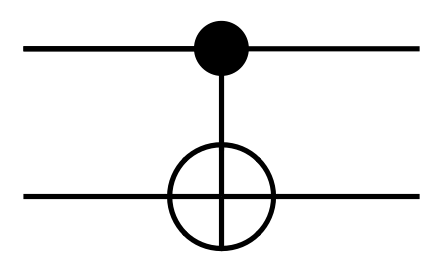
\includegraphics[width=0.15\linewidth]{gfx/CNOT_gate}\\ 
%         Toffoli & $\begin{pmatrix}
%             \mathbb{1}_6 & 0 \\
%             0 & X
%         \end{pmatrix}$ & 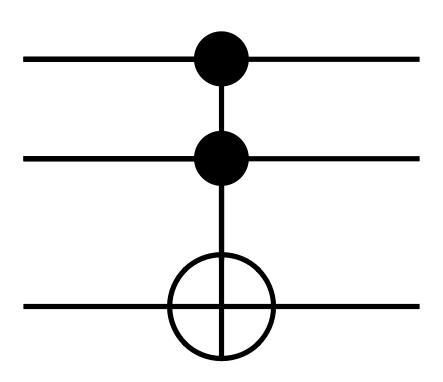
\includegraphics[width=0.15\linewidth]{gfx/Toffoli_gate}\\ 
%         nCNOT & $\begin{pmatrix}
%             \mathbb{1}_{2^n-2} & 0 \\
%             0 & X
%         \end{pmatrix}$ & \\ 
%         H & $\frac{1}{\sqrt{2}}\begin{pmatrix}
%             1 & 1 \\
%             1 & -1
%         \end{pmatrix}$ & 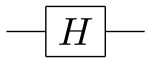
\includegraphics[width=0.15\linewidth]{gfx/150px-Hadamard_gate} \\ 
%         \hline
%     \end{tabular}
%     \caption{Porte logiche quantistiche}
%     \label{table:porte}
% \end{table}


